% Beinhaltet Empfänger und Diskrete Signale

\section{Empfänger} 
\subsection{Envelope Detektor (Hüllkurvendetektor)}
\begin{tabular}{ll}
 \addtolength{\jot}{2mm}
 \parbox{8cm}{Der Envelopen Demodulatoren können nur bei amplitudenmodulierte Signale verwendet werden. Um z.B. ein Amplitudenmoduliertes Signal zu demodulieren wird nur die positive Häfte eines zwei Seitenband AM Signal genommen und eine Hüllkurve über die Ausgangsfunktion gebildet. Das Ausgangssignal ist dann propotional zum modulierten Signal
}&
 \parbox{5cm}{
 \begin{tikzpicture}

\node[dspnodeopen,dsp/label=above] 					(c2) {$r(t)$}; 
\node[dspfilter, right= of c2]                    	(c3) {Envelope};
\node[dspnodeopen,, right= of c3, dsp/label=above] 	(c4) {$z(t)$};

\foreach \i [evaluate = \i as \j using int(\i+1)] in {2,...,3} \draw[dspconn] (c\i) -- (c\j);
\end{tikzpicture}}
\end{tabular}\\~
\vspace{6pt}
\begin{tabular}{lll}
 \addtolength{\jot}{2mm}
 \parbox{6cm}{
 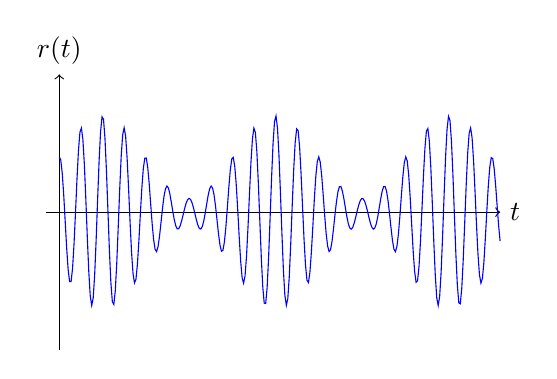
\begin{tikzpicture}[scale=0.70,
        dot/.style={circle,fill=blue,minimum size=3pt,inner sep=0pt,
            outer sep=-1pt},domain=0:4]
\draw[->] (-0.25,0) -- (8,0) node[right] {$t$};
 \draw[->] (0,-2.5) -- (0,2.5) node[above] {$r(t)$};

\draw[color=blue, domain=0:8, samples=300]   plot(\x,{((0.75*sin(2*\x r)+1)*(cos(16*\x r))});
      
\end{tikzpicture}\\
}&

 \parbox{6cm}{
 \begin{tikzpicture}[scale=0.70,
        dot/.style={circle,fill=blue,minimum size=3pt,inner sep=0pt,
            outer sep=-1pt},domain=0:4]
\draw[->] (-0.25,0) -- (8,0) node[right] {$t$};
 \draw[->] (0,-0.25) -- (0,2.5) node[above] {$z(t)$};

\draw[color=red, domain=0:8, samples=300]   plot(\x,{((0.75*sin(2*\x r)+1)}); 
         
\end{tikzpicture}\\ 
 }
\end{tabular}\\~
\vspace{6pt}
\textbf{1. Beispiel:} \quad Man zeige, dass ein Großhub-FM-Signal mit Hilfe einer Kaskade aus Differentiation und einem Enveloppendemodulator detektiert werden kann.
\begin{tabular}{ll}
 \addtolength{\jot}{2mm}
 \parbox{5cm}{
 \begin{eqnarray*}
 r(t) &= A \cdot cos(\omega_0t + \varphi(t))
 \end{eqnarray*}
}&
 \parbox{3cm}{
 \begin{tikzpicture}

\node[dspnodeopen,dsp/label=above] 					(c0) {$r(t)$};  
\node[dspfilter, right= of c0]                    	(c1) {$\frac{d}{dt}$};
\node[dspfilter, right= of c1]                    	(c2) {Envelope};
\node[dspnodeopen,, right= of c2, dsp/label=above] 	(c3) {$z(t)$};

\foreach \i [evaluate = \i as \j using int(\i+1)] in {0,1,...,2} \draw[dspconn] (c\i) -- (c\j);
\node (note1) at (3,0.5)  {$y(t)$};
\end{tikzpicture}}
\end{tabular}\\~
 \begin{eqnarray*}
 y(t) &= \dfrac{d}{dt}r(t) = A \cdot \left(\omega_0t + \underbrace{\dfrac{d\varphi(t)}{dt}}_{= \Delta \omega s_1(t)}\right)(-sin)\left(\omega_0t + \varphi(t) \right) = -A \cdot \omega_0 \left(1+ \dfrac{\Delta \omega s_1(t)}{\omega_0} \right) sin\left(\omega_0t + \varphi(t) \right)  \\
&\text{Enveloppen Demodulator} \Rightarrow z(t) \sim 1+ms_1(t) \hat{=} A(t) \qquad \qquad \vert \underbrace{\dfrac{\Delta \omega}{\omega_0}}_{=m} s_1(t) < 1 \vert
 \end{eqnarray*}\\
 \textbf{2. Beispiel:} \quad Gegeben sei ein allgemeines PM-Signal x(t) mit dem Informationstragenden Signal $s(t)$. Dann kann das Signal demoduliert werden mit Hilfe eines Produktdemodulator und einem Enveloppendetektor.
\begin{tabular}{ll}
 \addtolength{\jot}{2mm}
 \parbox{7cm}{
 \begin{eqnarray*}
 x(t) &=& A \cdot cos(2\pi f_0 t + m s_1(t))\\
 y(t) &=& A \cdot cos(2\pi f_0 t + m s_1(t))\cdot cos(2\pi f_0 t)\\
  &=& \frac{A}{2} \cdot cos(4\pi f_0 t + m s_1(t)) + \frac{A}{2} cos(2\pi f_0 t)\\
  TPF &\Rightarrow& \frac{A}{2} \cdot cos(m s(t)) \Rightarrow  r(t) = \frac{A}{2} \vert cos(ms(t)) \vert \neq \beta + \alpha s(t)
 \end{eqnarray*}
}&
 \parbox{3cm}{
 \begin{tikzpicture}[scale=0.7]
\node[dspnodeopen,dsp/label=above] 					(c0) {$x(t)$}; 
\node[dspmixer, right= of c0]   					(c1) {}; 
\node[dspfilter, right= of c1]                    	(c2) {Envelope};
\node[dspnodeopen,, right= of c2, dsp/label=above] 	(c3) {$r(t)$};
\node[dspnodeopen, above= of c1, dsp/label=right] 	(c4) {$cos(2\pi f_0 t)$};

\foreach \i [evaluate = \i as \j using int(\i+1)] in {0,1,...,2} \draw[dspconn] (c\i) -- (c\j);
\draw[dspconn] (c4) -- (c1);
\node (note1) at (2.5,0.25)  {$y(t)$};
\end{tikzpicture}}
\end{tabular}\\~
 Die Aussage das das Signal r(t) auf einer linearen mit s(t) zusammenhängt ist falsch. 
\subsection{AWGN-Kanäle}
\begin{tabular}{ll}
 \addtolength{\jot}{2mm}
 \parbox{6cm}{
Im Fall der LTI-Systeme wird das Signal am Empfänger als Faltung des gesendeten Informationssignals mit der Eigenschaft des Übertragungskanals dargestellt. Im Fall der realen Systeme wird das gesendete Informationssignal noch mit einem Rauschen überlagert. Dieses Rauschen wird als AWGN (additive white gaussian noise) bezeichnet und ist durch die Normalverteilung (Gausverteilung) geprägt. Es gibt Störungen durch Interferenzen mit anderen Signalen ($\omega(t)$) und thermisches Rauschen des Verstärkers ($n(t)$).}&
 \parbox{6cm}{
\begin{tikzpicture}[scale=0.7]
\node[dspnodeopen,dsp/label=above] 					(c0) {$s(t)$}; 
\node[dspfilter, right= of c0]   					(c1) {$h(\tau)$}; 
\node[dspadder, right= of c1]                    	(c2) {};
\node[dspadder, right= of c2]                    	(c3) {};
\node[dspnodeopen,, right= of c3, dsp/label=above] 	(c4) {$r(t)$};
\node[dspnodeopen, above= of c2, dsp/label=right] 	(c5) {$\omega(t)$};
\node[dspnodeopen, above= of c3, dsp/label=right] 	(c6) {$n(t)$};

\foreach \i [evaluate = \i as \j using int(\i+1)] in {0,1,...,3} \draw[dspconn] (c\i) -- (c\j);
\draw[dspconn] (c5) -- (c2);
\draw[dspconn] (c6) -- (c3);
\node (note1) at (4.25,0.45)  {$p(t)$};
\end{tikzpicture}
\vspace{6pt}\\~
In einem idealen Kanal ist $h(t) = \delta(t)$ und die Interferenz ist nicht vorhanden. Somit ist $p(t) = s(t)$, $\omega(t) = 0$ und daraus resultiert $r(t) = s_m(t) + n(t)$ mit $n(t)$ als stochasticher Prozess der unabhängig von $s(t)$ ist.}
\end{tabular}\\~
\vspace{6pt}\\
Das Rauschen kann im Signalraum $\mathbb{S}$, der von der Menge N orthogonalen Basen $f_n(t)$ aufgespannt wird. Graphisch dargestellt mit der Dimension $N=3$ und $s_m(t)$ aus $1 \leqslant m \leqslant M = 2$, welche antipodal aufgespannt sind:\\
\begin{tabular}{ll}
 \addtolength{\jot}{2mm}
 \parbox{7cm}{
  \begin{tikzpicture}[scale=0.75, dotb/.style={circle,fill=blue,minimum size=4pt,inner sep=0pt, outer sep=-1pt}]    
     
\draw[->, thick] (0,0,0) -- (4,0,0) node[anchor=north east, right=1mm]{$f_1$};
\draw[dashed, thick] (0,0,0) -- (-4,0,0);
\draw[->, thick] (0,0,0) -- (0,3,0) node[anchor=north west, left=1mm]{$f_2$};
\draw[dashed, thick] (0,0,0) -- (0,-3,0);
\draw[->, thick] (0,0,0) -- (0,0,3) node[anchor=south, right=1mm, below=1mm]{$f_3$};
\draw[dashed, thick] (0,0,0) -- (0,0,-3);

\draw[->, color=red] (0,0,0) -- (-2,0,0) node[anchor=north east, right=1mm, above=10mm] {$s_1(t)$};
\draw[->, color=blue] (0,0,0) -- (2,0,0) node[anchor=north east, right=1mm, above=10mm] {$s_2(t)$};

\end{tikzpicture}

}&
 \parbox{5cm}{Deutlich zu sehen ist das der Rauschprozess nicht nur in der Signalbasis, sondern in allen Basen verteilt ist. Die Rauschanteile sind zudem in jeder Dimension unabhängig, daher sollten für die Signaldetektion nicht mehr Dimensionen als nötig betrachtet werden. Die maximale Fehlerwarscheinlichkeit bei AWGN Kanälen ist 50\%, da bei 100\% alles falsch wäre und somit das richtige Signal die Invertierung des erkannten Signals ist.

}
\end{tabular}\\~
\subsection{Signal Demodulator}
\begin{center}
 \begin{tikzpicture}[scale=0.75]
\node[dspnodeopen,dsp/label=above] 					(c0) {$r(t)$};
\draw[dspconn] (c0) -- (c1); 
\node[dspnodefull, right= of c0]   					(c1) {}; 

\node[coordinate, above= of c1]                    	(c2) {};
\node[coordinate, above= of c2]                    	(c3) {};
\draw[dspline] (c1) -- (c3);
\node[dspmixer, right= of c3]                    	(c4) {};
\draw[dspconn] (c3) -- (c4);
\node[dspnodeopen, above= of c4, dsp/label=right] 	(c9) {$f_1(t)$};
\draw[dspconn] (c9) -- (c4);
\node[dspfilter, right= of c4]						(m1) {$\int_0^T () dt$};
\draw[dspconn] (c4) -- (m1);
\node[dspnodeopen,dsp/label=above, right= of m1] 	(m2) {};
\draw[decorate, decoration=switch] 					(m1) -- ++(m2);
\node[dspnodeopen,, right= of m2, dsp/label=above] (c11) {$r_1(t)$};
\draw[dspconn] (m2) -- (c11);

\node[coordinate, below= of c1]                    	(c5) {};
\node[coordinate, below= of c5]                    	(c6) {};
\draw[dspline] (c1) -- (c6);
\node[dspmixer, right= of c6]                    	(c7) {};
\draw[dspconn] (c6) -- (c7);
\node[dspnodeopen, above= of c7, dsp/label=right] 	(c10) {$f_3(t)$};
\draw[dspconn] (c10) -- (c7);
\node[dspfilter, right= of c7]						(m3) {$\int_0^T () dt$};
\draw[dspconn] (c7) -- (m3);
\node[dspnodeopen,dsp/label=above, right= of m3] 	(m4) {};
\draw[decorate, decoration=switch] 					(m3) -- ++(m4);
\node[dspnodeopen,, right= of m4, dsp/label=above] (c16) {$r_3(t)$};
\draw[dspconn] (m4) -- (c16);

\node[dspmixer, right= of c1]                    	(c8) {};
\draw[dspconn] (c1) -- (c8);
\node[dspnodeopen, above= of c8, dsp/label=right] 	(c11) {$f_2(t)$};
\draw[dspconn] (c11) -- (c8);
\node[dspfilter, right= of c8]						(m5) {$\int_0^T () dt$};
\draw[dspconn] (c8) -- (m5);
\node[dspnodeopen,dsp/label=above, right= of m5] 	(m6) {};
\draw[decorate, decoration=switch] 					(m5) -- ++(m6);
\node[dspnodeopen,, right= of m6, dsp/label=above] (c15) {$r_2(t)$};
\draw[dspconn] (m6) -- (c15);
\end{tikzpicture}\\
\end{center}
\vfill\columnbreak
\begin{tabular}{ll}
 \addtolength{\jot}{2mm}
 \parbox{7cm}{Der abgebildete \textbf{Korrelations Demodulatior} versucht die empfangenen Signale auf die Basen zu projizieren. Hierzu hat der Dektektor die einzelnen Basen $f_1(t), f_2(t), f_3(t), ...$ zur Verfügung. Das Empfangssignal ist wie folgt definiert: $r(t) = s_m + n$ für $m = 1,2,3,..,M$. Das Empfangssignal $r(t)$ ist ein Zufallsvektor, da dieser von dem Rauschvektor $n$ abhängt. Allgemein kann für jeden der $k$ Ausgänge gesagt werden:\\}&
 \parbox{5cm}{
\begin{eqnarray*}
r_k &=& \int^T_0 r(t) \cdot f_k(t) dt \\
 &=& \int^T_0 s(t) \cdot f_k(t) dt + \int^T_0 n(t) \cdot f_k(t) dt \\
 &=& s_{mk} + n_k
\end{eqnarray*}
}
\end{tabular}\\~
\begin{tabular}{ll}
 \addtolength{\jot}{2mm}
 \parbox{5cm}{
Eine weitere Detektionsart ist der sogenannte \textbf{Matched Filter} oder \textbf{signalangepasster Filter}, dieser basiert auf dem gleichen Prinzip des Korrelationsdemodulators, aber der Aufbau wird vereinfacht. Bei der Verwendung dieser Filter wird als Impulsantwort das spiegelverkehrte Signal geliefert. Durch diese Vereinfachung ist der Signal-Rausch-Abstand (SNR) geringer. Durch die Verwendung des angepassten Filters $h_i$ und \textit{Abtastung} bei $kT$ wird eine Korrelation des Eingangssignals mit dem Basissignal $f_i$ erzeugt.}&
 \parbox{7cm}{
\begin{tikzpicture}[scale=1]
\node[dspnodeopen,dsp/label=above] 					(c0) {$r(t)$}; 
\node[dspfilter, right= of c0]						(c1) {$h_i(t)$};
\node[dspnodeopen,dsp/label=above, right= of c1] 	(c2) {};
\node[dspnodeopen,dsp/label=above, right= of c2] 	(c3) {};
\draw[decorate, decoration=switch] 					(c2) -- ++(c3);
\node[dspnodeopen,dsp/label=above, right= of c3] 	(c4) {$y_i(T)$}; 

\draw[dspline] (c0) -- (c1);
\draw[dspline] (c1) -- (c2);
\draw[dspline] (c3) -- (c4);
\end{tikzpicture}\\
\begin{eqnarray*}
h_i(t) &=& f_i(T-t) \qquad \text{Signalangepasster Filter auf $r(t)$} \\
y_i(t) &=& r(t) \ast h_i(t) = \int_\mathbb{R} r(\tau) h_i(t - \tau) d\tau \\
&=& \int_\mathbb{R} r(\tau) f_i(T-t-\tau) d\tau \\
y(T) &=& \int_\mathbb{R} r(\tau) f_i(\tau) d\tau = <r(t), f_i(t)> = r_i
\end{eqnarray*}
}
\end{tabular}\\
\vspace{24pt}
\textbf{Beispiel:} \quad Es sei $r(t) = s(t) + n(t)$ ein empfangenes Signal mit Rauschsignal $n(t)$ eines AWGN mit Leistungspektraldichte $\frac{N_0}{2}$ und $s(t) = A \cdot \left(p(t) + p(t-2)\right)$ mit $p(t) = rect(2t-1)$.\vspace{6pt}\\~
\begin{tabular}{ll}
 \addtolength{\jot}{2mm}
 \parbox{5cm}{
  \begin{tikzpicture}[scale=1,domain=0:3.75, dot/.style={circle,fill=black,minimum size=3pt,inner sep=0pt,           outer sep=-1pt}]
\draw[->] (-0.25,0) -- (3.75,0) node[right] {$t$};
\draw[->] (0,-0.25) -- (0,1.5) node[above] {$s(t)$};

\draw[color=blue] (0,1) -- (1,1);;
\draw[dashed, color=blue] (1,1) -- (1,0);

\draw[color=blue] (2,1) -- (3,1);
\draw[dashed, color=blue] (2,1) -- (2,0);
\draw[dashed, color=blue] (3,1) -- (3,0);

\draw[thick] (1,-1.5pt) -- (1,1.5pt) node[below] {$1$};
\draw[thick] (2,-1.5pt) -- (2,1.5pt) node[below] {$2$};
\draw[thick] (3,-1.5pt) -- (3,1.5pt) node[below] {$3$};
\draw[thick] (-1.5pt,1) -- (1.5pt,1) node[left] {$A$};
\end{tikzpicture}}&
 \parbox{7cm}{
 Signalangepasster Filter mit:
 \begin{eqnarray*}
\text{Varianz: } \sigma_i^2 &=& \frac{N_0}{2} \\
\text{Erwartungswert: } \mu &=& \vec{s} \\
s(t) &=& A \cdot \left[rect(2t-1) + rect(2t-3) \right]  
 \end{eqnarray*}

}
\end{tabular}\\~
\vspace{6pt}
\begin{tabular}{ll}
 \addtolength{\jot}{2mm}
 \parbox{4.5cm}{
  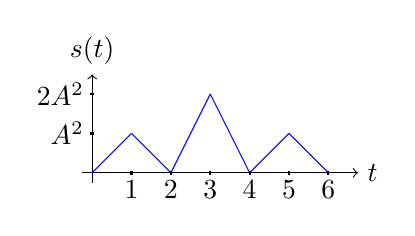
\begin{tikzpicture}[scale=0.5,domain=0:3.75, dot/.style={circle,fill=black,minimum size=3pt,inner sep=0pt,           outer sep=-1pt}]
\draw[->] (-0.25,0) -- (6.75,0) node[right] {$t$};
\draw[->] (0,-0.25) -- (0,2.5) node[above] {$s(t)$};

\draw[color=blue] (0,0) -- (1,1);
\draw[color=blue] (1,1) -- (2,0);
\draw[color=blue] (2,0) -- (3,2);
\draw[color=blue] (3,2) -- (4,0);
\draw[color=blue] (4,0) -- (5,1);
\draw[color=blue] (5,1) -- (6,0);


\draw[thick] (1,-1.5pt) -- (1,1.5pt) node[below] {$1$};
\draw[thick] (2,-1.5pt) -- (2,1.5pt) node[below] {$2$};
\draw[thick] (3,-1.5pt) -- (3,1.5pt) node[below] {$3$};
\draw[thick] (4,-1.5pt) -- (4,1.5pt) node[below] {$4$};
\draw[thick] (5,-1.5pt) -- (5,1.5pt) node[below] {$5$};
\draw[thick] (6,-1.5pt) -- (6,1.5pt) node[below] {$6$};
\draw[thick] (-1.5pt,1) -- (1.5pt,1) node[left] {$A^2$};
\draw[thick] (-1.5pt,2) -- (1.5pt,2) node[left] {$2A^2$};
\end{tikzpicture}}&
 \parbox{6cm}{
Das Ausgangssignal des Filters, wenn der Filter an das Signal angepasst ist $h(t) = s(t)$
 \begin{eqnarray*}
y(t) &=& A \left[p(t)+ p(t-2) \right] \ast  A \left[p(t)+ p(t-2) \right]\\
  &=& A^2 \left[\underbrace{p(t) \ast p(t)}_{\triangle(t)} + 2\underbrace{p(t) \ast p(t-2)}_{\triangle(t-3)} + \underbrace{p(t-2) \ast p(t-2)}_{\triangle(t-5)}  \right]\\ 
  &=& A^2 \left[ \triangle(t) + 2\triangle(t-3) + \triangle(t-5) \right] 
 \end{eqnarray*}}
\end{tabular}
\vspace{6pt}
\\ Der Erwartungswert der Zufallsvariablen $r(t)$ bei $T=3$ und somit ist der Erwartungswert von $s = 2A^2$. Das Rauschen ist mittelwertlos und normalverteilt mit der Varianz $\frac{N_0}{2}$. Zudem gilt $r(t) = s(t) - n(t) \Leftrightarrow n(t) = r(t) - s(t)$.
\begin{eqnarray*}
\sigma^2 &=& E \left( (r-s)^2 \right) = E \left( n^2 \right) = E \left( \int_\mathbb{R} n(t) \cdot s(t) dt \cdot \int_\mathbb{R} n(\tau) \cdot s(\tau) d\tau \right) \\
&=& E \left( \int_\mathbb{R}  \int_\mathbb{R} n(t) n(\tau) s(t) s(\tau) dt d\tau \right)
= \int \int \underbrace{ E\left( n(t) n(\tau) \right)}_{\frac{N_0}{2} \delta(t-\tau)} s(\tau) s(t) dt d\tau \\
&=& \int \int \frac{N_0}{2} \delta(t-\tau) s(\tau) s(t) dt d\tau = \frac{N_0}{2} \underbrace{\int s(t) s(t) dt}_\text{Energie} = \frac{N_0}{2} \cdot 2A^2 = N_0 A^2 
\end{eqnarray*}
\subsection{Signal Detektor}
\begin{tabular}{ll}
 \addtolength{\jot}{2mm}
 \parbox{7cm}{Nachdem das Empfangssignal $r(t)$ in seine einzelnen Komponenten $r_1(t), r_2(t), ...$ aufgeteilt wurde, kann nun entschieden werden, welches Signal $s_1(t), s_2(t),...$ gesendet wurde. Hierfür wird der Vektorraum $\mathbb{R}^N$ portioniert in Teilmengen $R(s_k)$, welche als Entscheidungsräume bezeichnet werden. Es wird sich genau dann für ein $s_k$ entschieden, wenn das Empfangssignal $r$ in einem Entscheidungsraum $R(s_k)$ liegt.}&
 \parbox{7cm}{
 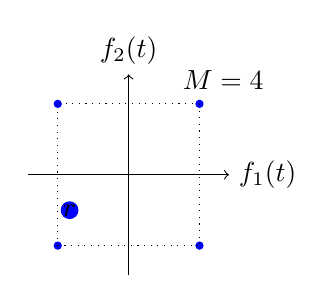
\begin{tikzpicture}[scale=0.3, dot/.style={circle,fill=blue,minimum size=3pt,inner sep=0pt,outer sep=-1pt}]
\draw[->] (-4.25,0) -- (4.25,0) node[right] {$f_1(t)$};
\draw[->] (0,-4.25) -- (0,4.25) node[above] {$f_2(t)$};

\node[dot] at (3,3)(int1) {};
\node[dot] at (3,-3)(int1) {};
\node[dot] at (-3,3)(int1) {};
\node[dot] at (-3,-3)(int1) {};

\draw[dotted] (3,3) -- (3,-3);
\draw[dotted] (3,3) -- (-3,3);
\draw[dotted] (-3,-3) -- (3,-3);
\draw[dotted] (-3,-3) -- (-3,3);

\node[dot] at (-2.5,-1.5)(int1) {$r$};

\node (note1) at (4,4)  {$M=4$};
\end{tikzpicture}}
\end{tabular}\\~
\begin{tabular}{ll}
 \addtolength{\jot}{2mm}
 \parbox{4.5cm}{
 Wenn $p(r,s_k)$ die Wahrscheinlichkeitsdichte von $r$, wenn $s_k$ gesendet wurde, so ist $P(r \in R(s_k) \vert s_k \text{ gesendet})$ und somit ist die bedingte Fehlerwahrscheinlichkeit $P(Fehler\vert s_k \text{ gesendet})$ . Die Gesamtfehlerwahrscheinlichkeit ist $P(Fehler)$. Die Entscheidungsräume sind wichtig um die Gesamtfehlerwahrscheinlichkeit minimal zu halten. Sind die Signalwahrscheinlichkeiten $P(s_k) = \frac{1}{M}$ gleich, so kann man hierfür das Maximum-Likelihood Kriterium verwenden}&
 \parbox{7cm}{
 \begin{eqnarray*}
P(r \in R(s_k) \vert s_k \text{ gesendet}) &=& \int_{R(s_k)} p(r \vert s_k)  dr \\
P(\text{Fehler} \vert s_k \text{ gesendet}) &=& 1 - \int_{R(s_k)} p(r \vert s_k)  dr \\
P(\text{Fehler}) &=& \sum_{k=1}^M P(s_k) \cdot P(\text{Fehler} \vert s_k \text{ gesendet}) \\
\text{ML:~} p(r\vert s_k) &=& \max_{i = 1,...,M} p(r \vert s_i)
 \end{eqnarray*}}
\end{tabular}\\~ 
\vspace{6pt}
\\
\textbf{1. Beispiel:} \quad Von einer mittelwertlosen, normalverteilten Wahrscheinlichkeitsgröße sei bekannt, dass die Varianz den Wert $\sigma_1^2 = 1$ und $\sigma_2^2 = 4$ mit jeweils der Wahrscheinlichkeit $\frac{1}{2}$ annehmen kann.\\
\vspace{6pt}
\begin{tabular}{ll}
 \addtolength{\jot}{2mm}
 \parbox{4cm}{
\begin{tikzpicture}
\begin{axis}[every axis plot post/.append style={
  mark=none,domain=-4:4,samples=50,smooth},									 % All plots: from -2:2, 50 samples, smooth, no marks
  axis x line*=bottom, 														% no box around the plot, only x and y axis
  axis y line*=middle, 												% the * suppresses the arrow tips
  enlargelimits=upper,
  xlabel={$r$},
  ylabel={$P$}, scale=0.5] 													% extend the axes a bit to the right and top
  \addplot {gauss(0,1)};
  \addplot {gauss(0,4)};
\end{axis}
\end{tikzpicture}
}&
 \parbox{7cm}{ Die Wahrscheinlichkeitsdichten sind mit $i = 1,2$
 \begin{eqnarray*}
 p(r \vert \sigma_i)&=& \frac{1}{\sqrt{2 \pi \sigma^2_i}} e^{\frac{- r^2}{2 \sigma^2_i}} 
 \end{eqnarray*}
 Die blaue Kurve ist mit Varianz $\sigma_1^2$ und die rote Kurve ist mit $\sigma_2^2$. Mit dem dem Maximum Likelihood Kriterium werden die Schnittpunkte so festgelegt, das im äußeren Bereich die rote Kurve und im inneren Bereich die blaue Kurve als Entscheidungsraum festgelegt wird.}
\end{tabular}\\
 \begin{eqnarray*}
 P(r \vert \sigma_1^2) = \frac{1}{\sqrt{2 \pi \sigma^2_1}} e^{\frac{- r^2}{2 \sigma^2_1}}   &\geq& p(r \vert \sigma_2^2) = \frac{1}{\sqrt{2 \pi \sigma^2_2}} e^{\frac{- r^2}{2 \sigma^2_2}} \\ 
ln ( \frac{1}{\sqrt{2 \pi \sigma^2_1}} ) - \frac{- r^2}{2 \sigma^2_1} &\geq&   ln ( \frac{1}{\sqrt{2 \pi \sigma^2_2}} ) - \frac{- r^2}{2 \sigma^2_2} \\
r^2 \left( \frac{1}{2\sigma_2^2} - \frac{1}{2\sigma_1^2} \right) &\geq& ln \left( \frac{\sigma_1}{\sigma_2} \right) \\
r^2 \left( \frac{1}{2\sigma_1^2} - \frac{1}{2\sigma_2^2} \right) &\leq& ln \left( \frac{\sigma_2}{\sigma_1} \right) \\
r^2 \left( \frac{1}{2} - \frac{1}{8} \right)  &\leq& ln(2)\\
\vert r \vert &=& \sqrt{\frac{8 ln(2)}{3}} 
 \end{eqnarray*}\\
\begin{tabular}{ll}
 \addtolength{\jot}{2mm}
 \parbox{5cm}{
  Die Entscheidungsräume sind somit bei $R(\sigma_1) = [-r_0;r_0]$ und bei $R(\sigma_2) = ( -\inf ; r_0] \cup [r_0 ; \inf)$ mit $r_0 = \sqrt{\frac{8 ln(2)}{3}}$. Die Fehler können mit der Q Funktion ermittelt werden. Die Gesamtfehlerwahrscheinlichkeit liegt dann bei $\approx 0,336$.}&
 \parbox{5cm}{
 \begin{eqnarray*}
 P(\text{Fehler} \vert \sigma_1^2) &=& 2Q(\frac{r_0}{\sigma_1} \approx 2Q(1,4) \approx 0,16152 \\
  P(\text{Fehler} \vert \sigma_2^2) &=& 1 - 2Q(\frac{r_0}{\sigma_2} \approx 1- 2Q(0.7) \approx 0,51061 \\
  P(\text{Fehler}) &=& \frac{1}{2} P(\text{Fehler} \vert \sigma_1^2) + \frac{1}{2} P(\text{Fehler} \vert \sigma_2^2)
 \end{eqnarray*}

}
\end{tabular}
\\
\vspace{12pt}
\textbf{2. Beispiel:}
\vfill\columnbreak
\textbf{3. Beispiel:} \quad Die Nachrichtensignale $s_1(t), s_2(t)$ und $s_3(t)$ werden über einen AWGN-Kanal mit Leistungsspektraldichte $\frac{N_0}{2}$ übertragen. Dabei ist: $s_1(t) = rect(\frac{2t}{T}-1)$ und $s_2(t) = - s_3(t) = rect(\frac{4t}{T}-1) - rect(\frac{4t}{T}-3)$\\
\vspace{6pt}
\begin{tabular}{ll}
 \addtolength{\jot}{2mm}
 \parbox{4cm}{
\begin{tikzpicture}[scale=0.4] 
\draw[->] (-0.25,0) -- (2.5,0) node[right] {$t$};
\draw[->] (0,-1.5) -- (0,1.5) node[above] {$s_1(t)$};
	
\draw[dashed, color=red] (0,0) -- (0,1);
\draw[color=red] (0,1) -- (2,1);
\draw[dashed, color=red] (2,0) -- (2,1);
\end{tikzpicture}
\begin{tikzpicture}[scale=0.4] 
\draw[->] (-0.25,0) -- (2.5,0) node[right] {$t$};
\draw[->] (0,-1.5) -- (0,1.5) node[above] {$s_2(t)$};
	
\draw[dashed, color=red] (0,0) -- (0,1);
\draw[color=red] (0,1) -- (1,1);
\draw[dashed, color=red] (1,1) -- (1,-1);
\draw[color=red] (1,-1) -- (2,-1);
\draw[dashed, color=red] (2,0) -- (2,-1);
\end{tikzpicture} 
\begin{tikzpicture}[scale=0.4] 
\draw[->] (-0.25,0) -- (2.5,0) node[right] {$t$};
\draw[->] (0,-1.5) -- (0,1.5) node[above] {$s_3(t)$};
	
\draw[dashed, color=red] (0,0) -- (0,-1);
\draw[color=red] (0,-1) -- (1,-1);
\draw[dashed, color=red] (1,1) -- (1,-1);
\draw[color=red] (1,1) -- (2,1);
\draw[dashed, color=red] (2,0) -- (2,1);
\end{tikzpicture}\\
 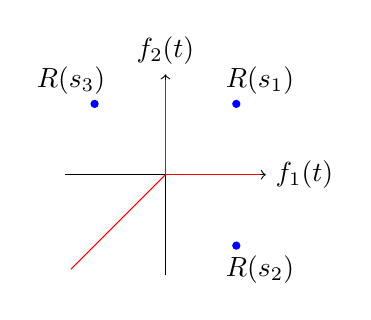
\begin{tikzpicture}[scale=0.3, dot/.style={circle,fill=blue,minimum size=3pt,inner sep=0pt,outer sep=-1pt}]
\draw[->] (-4.25,0) -- (4.25,0) node[right] {$f_1(t)$};
\draw[->] (0,-4.25) -- (0,4.25) node[above] {$f_2(t)$};

\node[dot] at (3,3)(int1) {};
\node[dot] at (3,-3)(int1) {};
\node[dot] at (-3,3)(int1) {};

\draw[color=red] (0,0) -- (-4,-4);
\draw[color=red] (0,0) -- (4,0);
\draw[color=red] (0,0) -- (0,4);

\node (note1) at (4,4)  {$R(s_1)$};
\node (note1) at (-4,4)  {$R(s_3)$};
\node (note1) at (4,-4)  {$R(s_2)$};
\end{tikzpicture}}&
 \parbox{7cm}{Als orthonormale Basis könnten nun zwei Basen erstellt werden:\\
 \begin{eqnarray*}
 f_1(t) &=& \sqrt{\frac{2}{T}} \cdot rect \left( \frac{4t}{T} -1 \right) \\
  f_2(t) &=& \sqrt{\frac{2}{T}} \cdot rect \left( \frac{4t}{T} -3 \right)
\end{eqnarray*}
Aus diesen Basen können nun die Signale vollständig dargestellt werden:
 \begin{eqnarray*}
s_1(t) = \sqrt{\frac{T}{2}} \cdot f_1(t) + \sqrt{\frac{T}{2}} \cdot f_2(t)  \\
s_2(t) = \sqrt{\frac{T}{2}} \cdot f_1(t) - \sqrt{\frac{T}{2}} \cdot f_2(t)  \\
s_3(t) = - \sqrt{\frac{T}{2}} \cdot f_1(t) + \sqrt{\frac{T}{2}} \cdot f_2(t)  \\
\end{eqnarray*} 
Die Entscheidungsräume können nun grafisch dargestellt werden. Man sieht: $P(\text{Fehler} \vert s_1 \text{gesendet}) < P(\text{Fehler} \vert s_2 \text{gesendet}) = P(\text{Fehler} \vert s_3 \text{ gesendet})$ Somit ist $s_1$ am fehleranfälligsten.}
\end{tabular}\\
Für die bedingten Fehlerwahrscheinlichkeiten gilt für die drei Signale mit $\sigma^2 = \frac{N_0}{2}$:
\begin{eqnarray*}
 p(r \vert s_1)&=& \frac{1}{\sqrt{2 \pi \sigma^2}} exp(\frac{- \Vert r - s_1 \Vert^2}{2 \sigma^2})\\ &=& \frac{1}{\sqrt{2 \pi \sigma^2}} \int^{\infty}_0 exp(\frac{- \Vert r - \sqrt{\frac{T}{2}} \Vert^2}{2 \sigma^2} dr_1 \cdot \int^{\infty}_0 exp(\frac{- \Vert r - \sqrt{\frac{T}{2}} \Vert^2}{2 \sigma^2} dr_2 \\ &=& (1-Q(\frac{\sqrt{T/2}}{\sigma}))^2 = (1-Q(\sqrt{T/N_0}))^2 \\[6pt]
P(\text{Fehler} \vert s_1 \text{gesendet}) &=& 1-(1-Q(\sqrt{T/N_0}))^2 = (2-Q(\sqrt{T/N_0}))Q(\sqrt{T/N_0})
\end{eqnarray*}\\
Die Integration über die Ereignismenge $R(s_2)$ kann über die Betrachtung mit zwei Hilfsmengen $R^{'}_2 = \lbrace r \in \mathbb{R}^2: r_1 \geqslant 0, r_2 \leqslant 0 \rbrace$ und $R^{''}_2 = \lbrace r \in \mathbb{R}^2: r_2 \leqslant r_1 \rbrace$ Wegen der Symmetrie der Dichtefunktion und der Mengen gilt $P(r \in R(s_2) \vert s_2)$, dies kann Analog zu der Betrachtung von $P(r \in R(s_1) \vert s_1) = (1-Q(\sqrt{T/N_0}))^2$ gemacht werden. Bei der Berechung von $P(r \in R^{''}(s_2) \vert s_2)$ wird $R^{''}$ als Halbebene angesehen (Siehe Betrachtung Halbebene Stochastik).  Die Gerade $r_1 = r_2$ hat den Abstand $d = \sqrt{T}$, somit gilt $P(r \in R^{''}(s_2) \vert s_2) = 1-Q(\sqrt{2T/N_0}$.
\begin{eqnarray*}
P(\text{Fehler} \vert s_2 \text{ gesendet}) = \frac{1}{2}((2-Q(\sqrt{T/N_0})Q(\sqrt{T/N_0})+Q(\sqrt{2T/N_0})
\end{eqnarray*}
Durch die Symmetrie von $s_2$ und $s_3$ ergibt sich als Lösung:
\begin{eqnarray*}
P(\text{Fehler} \vert s_1 \text{ gesendet}) &\approx& 0.155 \\
P(\text{Fehler} \vert s_2 \text{ gesendet}) &\approx& 0.089 \\
P(\text{Fehler} \vert s_3 \text{ gesendet}) &\approx& 0.089 \\
P(\text{Fehler} &\approx& 0.111
\end{eqnarray*}
\section{Diskrete Signale} 
\subsection{diskrete Funktionen}
\begin{tabular}{ll}
 \addtolength{\jot}{2mm}
 \parbox{5cm}{
\begin{center}
 \textbf{Diracstoß}\\
\end{center}
 \begin{align*}
\delta[k] = \begin{cases} 1 \quad &k = 0\\[1em]
							0 \quad &\text{sonst}
	\end{cases}
 \end{align*}
 }&
 \parbox{6cm}{
 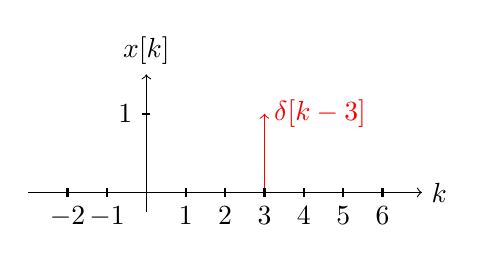
\begin{tikzpicture}[scale=1, dot/.style={circle,fill=black,minimum size=3pt,inner sep=0pt, outer sep=-1pt}]
	\draw[->] (-1.5,0) -- (3.5,0) node[right] {$k$};
    \draw[->] (0,-0.25) -- (0,1.5) node[above] {$x[k]$};
    
  	\draw[->, color=red] (1.5,0) -- (1.5,1)node [right] {$\delta[k-3]$};
	
	\draw[thick] (-1,-1.5pt) -- (-1,1.5pt) node[below=1mm] {$-2$};
	\draw[thick] (-0.5,-1.5pt) -- (-0.5,1.5pt) node[below=1mm] {$-1$};		
	\draw[thick] (0.5,-1.5pt) -- (0.5,1.5pt) node[below=1mm] {$1$};	
	\draw[thick] (1,-1.5pt) -- (1,1.5pt) node[below=1mm] {$2$};	
	\draw[thick] (1.5,-1.5pt) -- (1.5,1.5pt) node[below=1mm] {$3$};	
	\draw[thick] (2,-1.5pt) -- (2,1.5pt) node[below=1mm] {$4$};	
	\draw[thick] (2.5,-1.5pt) -- (2.5,1.5pt) node[below=1mm] {$5$};	
	\draw[thick] (3,-1.5pt) -- (3,1.5pt) node[below=1mm] {$6$};
	\draw[thick] (-1.5pt,1) -- (1.5pt,1) node[left=1mm] {$1$};
\end{tikzpicture}
 }
\end{tabular}\\ 
\begin{tabular}{ll}
 \addtolength{\jot}{2mm}
 \parbox{5cm}{
\begin{center}
 \textbf{Sprungfolge}\\
\end{center}
 \begin{align*}
\epsilon[k] = \begin{cases} 1 \quad &k \geq 0\\[1em]
							0 \quad &\text{sonst}
	\end{cases}\\
\epsilon[k] = \sum_{i=0}^\infty \delta[k-i]
 \end{align*}
 }&
 \parbox{6cm}{
 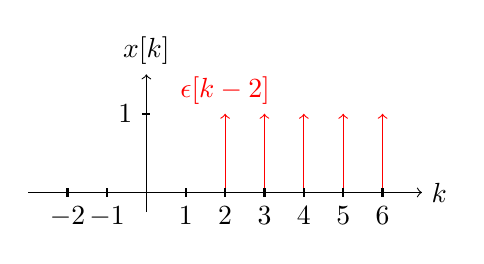
\begin{tikzpicture}[scale=1, dot/.style={circle,fill=black,minimum size=3pt,inner sep=0pt, outer sep=-1pt}]
	\draw[->] (-1.5,0) -- (3.5,0) node[right] {$k$};
    \draw[->] (0,-0.25) -- (0,1.5) node[above] {$x[k]$};
    
  	\draw[->, color=red] (1,0) -- (1,1)node [above] {$\epsilon[k-2]$};
  	\draw[->, color=red] (1.5,0) -- (1.5,1)node [right] {};
  	\draw[->, color=red] (2,0) -- (2,1)node [right] {};
  	\draw[->, color=red] (2.5,0) -- (2.5,1)node [right] {};
  	\draw[->, color=red] (3,0) -- (3,1)node [right] {};  	

	\draw[thick] (-1,-1.5pt) -- (-1,1.5pt) node[below=1mm] {$-2$};
	\draw[thick] (-0.5,-1.5pt) -- (-0.5,1.5pt) node[below=1mm] {$-1$};	  		
	\draw[thick] (0.5,-1.5pt) -- (0.5,1.5pt) node[below=1mm] {$1$};	
	\draw[thick] (1,-1.5pt) -- (1,1.5pt) node[below=1mm] {$2$};	
	\draw[thick] (1.5,-1.5pt) -- (1.5,1.5pt) node[below=1mm] {$3$};	
	\draw[thick] (2,-1.5pt) -- (2,1.5pt) node[below=1mm] {$4$};	
	\draw[thick] (2.5,-1.5pt) -- (2.5,1.5pt) node[below=1mm] {$5$};	
	\draw[thick] (3,-1.5pt) -- (3,1.5pt) node[below=1mm] {$6$};
	\draw[thick] (-1.5pt,1) -- (1.5pt,1) node[left=1mm] {$1$};
\end{tikzpicture}
 }
\end{tabular}\\
\begin{tabular}{ll}
 \addtolength{\jot}{2mm}
 \parbox{5cm}{
\begin{center}
 \textbf{Rechteckimpuls}\\
\end{center}
 \begin{align*}
rect_n[k] = \begin{cases} 1 \quad &0 \leq k \leq N-1\\[1em]
							0 \quad &\text{sonst}
	\end{cases}\\
rect_n[k] = \epsilon[k]-\epsilon[k-N] = \sum_{i=0}^{N-1} \delta[k-i]
 \end{align*}
 }&
 \parbox{6cm}{
 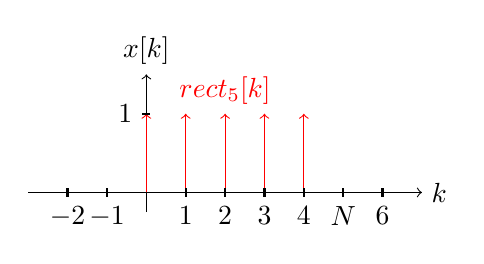
\begin{tikzpicture}[scale=1, dot/.style={circle,fill=black,minimum size=3pt,inner sep=0pt, outer sep=-1pt}]
	\draw[->] (-1.5,0) -- (3.5,0) node[right] {$k$};
    \draw[->] (0,-0.25) -- (0,1.5) node[above] {$x[k]$};
    
  	\draw[->, color=red] (0,0) -- (0,1)node [above] {};
  	\draw[->, color=red] (0.5,0) -- (0.5,1)node [right] {};
  	\draw[->, color=red] (1,0) -- (1,1)node [above] {$rect_5[k]$};
  	\draw[->, color=red] (1.5,0) -- (1.5,1)node [right] {};
  	\draw[->, color=red] (2,0) -- (2,1)node [right] {};  	

	\draw[thick] (-1,-1.5pt) -- (-1,1.5pt) node[below=1mm] {$-2$};
	\draw[thick] (-0.5,-1.5pt) -- (-0.5,1.5pt) node[below=1mm] {$-1$};	  		
	\draw[thick] (0.5,-1.5pt) -- (0.5,1.5pt) node[below=1mm] {$1$};	
	\draw[thick] (1,-1.5pt) -- (1,1.5pt) node[below=1mm] {$2$};	
	\draw[thick] (1.5,-1.5pt) -- (1.5,1.5pt) node[below=1mm] {$3$};	
	\draw[thick] (2,-1.5pt) -- (2,1.5pt) node[below=1mm] {$4$};	
	\draw[thick] (2.5,-1.5pt) -- (2.5,1.5pt) node[below=1mm] {$N$};	
	\draw[thick] (3,-1.5pt) -- (3,1.5pt) node[below=1mm] {$6$};
	\draw[thick] (-1.5pt,1) -- (1.5pt,1) node[left=1mm] {$1$};
\end{tikzpicture}
 }
\end{tabular}\\ \vspace{6pt}
\begin{tabular}{ll}
 \addtolength{\jot}{2mm}
 \parbox{5cm}{
\begin{center}
 \textbf{Signumfolge}\\
\end{center}
 \begin{align*}
sgn[k] = \begin{cases} 1 \quad &k > 0\\[1em]
						0 \quad &k = 0\\[1em]
							-1 \quad &k < 0
	\end{cases}\\
sgn[k] = \epsilon[k]-\epsilon[-k] = 2\epsilon[k]-1-\delta[k]
 \end{align*}
 }&
 \parbox{6cm}{
 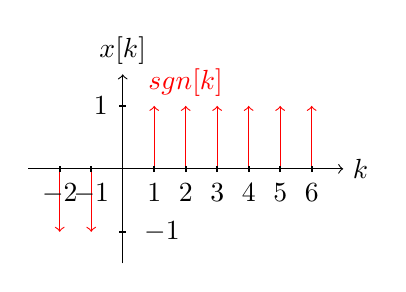
\begin{tikzpicture}[scale=0.8, dot/.style={circle,fill=black,minimum size=3pt,inner sep=0pt, outer sep=-1pt}]
	\draw[->] (-1.5,0) -- (3.5,0) node[right] {$k$};
    \draw[->] (0,-1.5) -- (0,1.5) node[above] {$x[k]$};
    
  	\draw[->, color=red] (-1,0) -- (-1,-1)node [above] {};
  	\draw[->, color=red] (-0.5,0) -- (-0.5,-1)node [right] {};
  	\draw[->, color=red] (0.5,0) -- (0.5,1)node [right] {};
  	\draw[->, color=red] (1,0) -- (1,1)node [above] {$sgn[k]$};
  	\draw[->, color=red] (1.5,0) -- (1.5,1)node [right] {};
  	\draw[->, color=red] (2,0) -- (2,1)node [right] {}; 
  	\draw[->, color=red] (2.5,0) -- (2.5,1)node [right] {};
  	\draw[->, color=red] (3,0) -- (3,1)node [right] {};  	

	\draw[thick] (-1,-1.5pt) -- (-1,1.5pt) node[below=1mm] {$-2$};
	\draw[thick] (-0.5,-1.5pt) -- (-0.5,1.5pt) node[below=1mm] {$-1$};	  		
	\draw[thick] (0.5,-1.5pt) -- (0.5,1.5pt) node[below=1mm] {$1$};	
	\draw[thick] (1,-1.5pt) -- (1,1.5pt) node[below=1mm] {$2$};	
	\draw[thick] (1.5,-1.5pt) -- (1.5,1.5pt) node[below=1mm] {$3$};	
	\draw[thick] (2,-1.5pt) -- (2,1.5pt) node[below=1mm] {$4$};	
	\draw[thick] (2.5,-1.5pt) -- (2.5,1.5pt) node[below=1mm] {$5$};	
	\draw[thick] (3,-1.5pt) -- (3,1.5pt) node[below=1mm] {$6$};
	\draw[thick] (-1.5pt,1) -- (1.5pt,1) node[left=1mm] {$1$};
	\draw[thick] (-1.5pt,-1) -- (1.5pt,-1) node[right=1mm] {$-1$};
\end{tikzpicture}}
\end{tabular}
\begin{tabular}{ll}
 \addtolength{\jot}{2mm}
 \parbox{5cm}{
\begin{center}
 \textbf{Energie}\\
\end{center}
Für periodische Signale reicht die Betrachtung der Periode $N_p$ bei beliebigen Startpunkt $k_0$. Ein Energiesignal ist kein Leistungssignal und umgekehrt, da die Leistung eines Energiesignals null ist.
 }&
 \parbox{6cm}{
 \begin{eqnarray*}
 E_x &=& \sum_{k = -\infty}^{\infty} [x[k]]^2 \quad \text{Energiesignal $E_x < \infty$}\\
 P_x &=& \lim_{n \rightarrow \infty} \frac{1}{2n+1} \sum_{k = -n}^{n} [x[k]]^2 \quad \text{mittlere Leistung}\\
 P_x &=& \frac{1}{N_p} \sum_{k = k_0}^{k_0 + N_p - 1}[x[k]]^2 \quad \text{period. Leistungssignal}
 \end{eqnarray*} }
\end{tabular}\\ \vspace{6pt}
\begin{tabular}{ll}
 \addtolength{\jot}{2mm}
 \parbox{5cm}{
\begin{center}
 \textbf{Skalarprodukt und Kreuzkorrelation}\\
\end{center}
Das innere Produkt mit sich selber ist die Energie des Signals. Die Signale sind orthogonal aufeinander, wenn das Innere Produkt null ergibt. Die Kreuzkorrelation wird mit einem um $K$ verschobenen bzw. Zeitlich verzögerten Anteil durchgeführt.
 }&
 \parbox{6cm}{
 \begin{eqnarray*}
< x[k] , y[k] > &=& \sum_{k = -\infty}^{\infty} x^*[k] y[k]\\
\varphi_{xy}^E [k] &=& < x[k], y[k+K] > = \sum_{k = -\infty}^{\infty} x^*[k] y[k+K]\\
\varphi_{xx}^E [k] &=& < x[k], x[k+K] > \quad \text{Autokorrelation}
 \end{eqnarray*} }
\end{tabular}\vspace{6pt}\\
Bei periodischen Signalen mit gemeinsamer Periode $N_p$ (gemeinsames Vielfache der einzelnen Perioden $N_x$ und $N_y$) mit beliebigem Startpunkt $k_0$:
\begin{eqnarray*}
\varphi_{xy}^{L} [k] &=& \frac{1}{N_p} \sum_{k = k_0}^{k_0 + N_p - 1}x^*[k] y[k+K]\\
\varphi_{xy} [k] &=& \varphi_{xy}^* [k]\\
\varphi_{xx} [k] &=& \varphi_{xx}^* [-k]
\end{eqnarray*}
Zudem gelten die unteren Bedingungen, da die relative Verschiebung von $k$ wichtig ist.\\ \vspace{6pt}
\textbf{Beispiel:}
\vspace{6pt}\\
\begin{tabular}{ll}
 \addtolength{\jot}{2mm}
 \parbox{6cm}{
 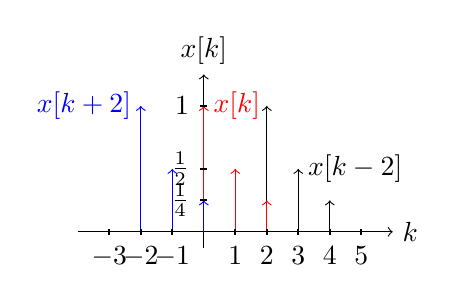
\begin{tikzpicture}[scale=0.8, dot/.style={circle,fill=black,minimum size=3pt,inner sep=0pt, outer sep=-1pt}]
	\draw[->] (-2,0) -- (3,0) node[right] {$k$};
    \draw[->] (0,-0.25) -- (0,2.5) node[above] {$x[k]$};
 
   	\draw[->, color=black] (1,0) -- (1,2)node [right] {};
  	\draw[->, color=black] (1.5,0) -- (1.5,1)node [right] {$x[k-2]$};
  	\draw[->, color=black] (2,0) -- (2,0.5)node [right] {};
    
  	\draw[->, color=red] (0,0) -- (0,2)node [right] {$x[k]$};
  	\draw[->, color=red] (0.5,0) -- (0.5,1)node [right] {};
  	\draw[->, color=red] (1,0) -- (1,0.5)node [right] {};

  	\draw[->, color=blue] (-1,0) -- (-1,2)node [left] {$x[k+2]$};
  	\draw[->, color=blue] (-0.5,0) -- (-0.5,1)node [right] {};
  	\draw[->, color=blue] (0,0) -- (0,0.5)node [right] {};	

	\draw[thick] (-1.5,-1.5pt) -- (-1.5,1.5pt) node[below=1mm] {$-3$};	
	\draw[thick] (-1,-1.5pt) -- (-1,1.5pt) node[below=1mm] {$-2$}; 
	\draw[thick] (-0.5,-1.5pt) -- (-0.5,1.5pt) node[below=1mm] {$-1$};	 		
	\draw[thick] (0.5,-1.5pt) -- (0.5,1.5pt) node[below=1mm] {$1$};	
	\draw[thick] (1,-1.5pt) -- (1,1.5pt) node[below=1mm] {$2$};	
	\draw[thick] (1.5,-1.5pt) -- (1.5,1.5pt) node[below=1mm] {$3$};	
	\draw[thick] (2,-1.5pt) -- (2,1.5pt) node[below=1mm] {$4$};	
	\draw[thick] (2.5,-1.5pt) -- (2.5,1.5pt) node[below=1mm] {$5$};	;
	\draw[thick] (-1.5pt,0.5) -- (1.5pt,0.5) node[left=1mm] {$\frac{1}{4}$};
	\draw[thick] (-1.5pt,1) -- (1.5pt,1) node[left=1mm] {$\frac{1}{2}$};
	\draw[thick] (-1.5pt,2) -- (1.5pt,2) node[left=1mm] {$1$};
\end{tikzpicture}
 }&
 \parbox{6cm}{
 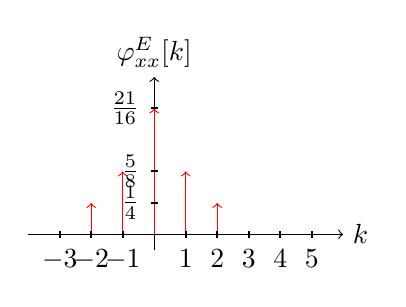
\begin{tikzpicture}[scale=0.8, dot/.style={circle,fill=black,minimum size=3pt,inner sep=0pt, outer sep=-1pt}]
	\draw[->] (-2,0) -- (3,0) node[right] {$k$};
    \draw[->] (0,-0.25) -- (0,2.5) node[above] {$\varphi_{xx}^E[k]$};
    
  	\draw[->, color=red] (-1,0) -- (-1,0.5)node [right] {};
  	\draw[->, color=red] (-0.5,0) -- (-0.5,1)node [right] {};
  	\draw[->, color=red] (0,0) -- (0,2)node [right] {};
  	\draw[->, color=red] (0.5,0) -- (0.5,1)node [right] {};  	
  	\draw[->, color=red] (1,0) -- (1,0.5)node [right] {};  	

	\draw[thick] (-1.5,-1.5pt) -- (-1.5,1.5pt) node[below=1mm] {$-3$};	
	\draw[thick] (-1,-1.5pt) -- (-1,1.5pt) node[below=1mm] {$-2$}; 
	\draw[thick] (-0.5,-1.5pt) -- (-0.5,1.5pt) node[below=1mm] {$-1$};	 		
	\draw[thick] (0.5,-1.5pt) -- (0.5,1.5pt) node[below=1mm] {$1$};	
	\draw[thick] (1,-1.5pt) -- (1,1.5pt) node[below=1mm] {$2$};	
	\draw[thick] (1.5,-1.5pt) -- (1.5,1.5pt) node[below=1mm] {$3$};	
	\draw[thick] (2,-1.5pt) -- (2,1.5pt) node[below=1mm] {$4$};	
	\draw[thick] (2.5,-1.5pt) -- (2.5,1.5pt) node[below=1mm] {$5$};	
	\draw[thick] (-1.5pt,0.5) -- (1.5pt,0.5) node[left=1mm] {$\frac{1}{4}$};
	\draw[thick] (-1.5pt,1) -- (1.5pt,1) node[left=1mm] {$\frac{5}{8}$};
	\draw[thick] (-1.5pt,2) -- (1.5pt,2) node[left=1mm] {$\frac{21}{16}$};
\end{tikzpicture}}
\end{tabular}
Man sieht, dass das Signal ein Energiesignal ist. $x[k]$ ist nicht periodisch.
\begin{eqnarray*}
E_x &=& \sum_{k \in \mathbb{Z}} [x[k]]^2 = 1^2 + \frac{1}{2^2} + \frac{1}{4^2} = \frac{21}{16} < \infty
\end{eqnarray*}
Die mittlere Leistung von $x[k]$ ist gleich Null.
\begin{eqnarray*}
\varphi_{xx}^E [k] &=& \sum_{k \in \mathbb{Z}} x[k]x[k+2] = 1 \cdot \frac{1}{4}\\
\varphi_{xx}^E [2] &=& \varphi_{xx}^E [-2]
\end{eqnarray*}
Die Korrelationsspitze bzw. das Maximum liegt bei $k=0$. Beispiel für solche Anwendungen ist bei der zeitlichen Synchronisation von WLAN. Hardware technisch kann dies über einen Differentiation (Vorzeichenänderung = Nulldurchgang) umgesetzt werden.
\subsection{z-Transformation}
Allgemein gilt für die Transformation und Rücktransformation folgender Satz:
\begin{eqnarray*}
x[k] &\laplace& X(z) = \sum_{k = - \infty}^{\infty} x[k] \cdot z^{-k} \qquad z \in \mathbb{C} \\ 
\delta[k+k_0] &\laplace& z^{k_0} 
\end{eqnarray*}
Desweiteren gelten noch folgende Rechenregeln und Definitionen:
\begin{tabular}{ll}
 \addtolength{\jot}{2mm}
 \parbox{5cm}{\begin{eqnarray*}
 \delta[k] &\laplace& 1\\
  \epsilon[k] &\laplace& \frac{z}{z-1} \quad \text{$\vert z \vert > 1$}\\
  \alpha^k \epsilon[k] &\laplace& \frac{z}{z-a} \quad \text{$\vert z \vert > \alpha$}\\
  \alpha_1 x_1[k] +   \alpha_2 x_2[k] &\laplace& \alpha_1 X_1(z) + \alpha_2 X_2(z) \\
  x[k] \ast y[k] &\laplace&  X(z) \cdot Y(z) \\
  \delta[k]  + 3 \delta[k-2]  &\laplace& 1 + \frac{3}{z^2}\\
  x[-k]  &\laplace& X\left( \frac{1}{z}\right) \\
  x^*[k]  &\laplace& X^*(z^*)\\
  x[k-k_0]  &\laplace&  X(z) \cdot z^{-k_0}
 \end{eqnarray*}
}
 &
 \addtolength{\jot}{2mm}
 \parbox{5cm}{\begin{eqnarray*}
\frac{a}{z^m} &\Laplace& a \delta[k-m]\\
\frac{z}{z-a} &\Laplace& a^k \epsilon[k]\\
\frac{1}{z-a} &\Laplace& a^{k-1} \epsilon[k-1]\\
\frac{z}{(z-a)^{m+1}} &\Laplace& \binom{k}{m} a^{k-m} \epsilon[k]\\
\text{Ableitung: } x[k] - x[k-1] &\laplace& X(z) \cdot \frac{z-1}{z}\\
\text{Integral: } \sum_{i=-\infty}^k x[i] &\laplace& X(z) \cdot \frac{z}{z-1}\\
\text{peri. Fortsetzung: } \sum_{i=0}^k x[k-iN] &\laplace& X(z) \cdot \frac{1}{1-z^{-N}}\\
\varphi^E_{xy} = x^*[k] \ast y[k] &\laplace& X^*\left(\frac{1}{z^*}\right) \cdot Y(z)
 \end{eqnarray*}}
\end{tabular}\\
\textbf{Rechenregeln für Reihen und Folgen zur z-Transformation}
\begin{tabular}{ll}
 \addtolength{\jot}{2mm}
 \parbox{7cm}{
 \begin{eqnarray*}
  \sum_{i=0}^n a^i &=& \frac{1-a^{n+1}}{1-a} = \frac{a^{n+1}-1}{a-1}  \quad a \neq 1\\
 \sum_{i=0}^{\infty} a^i &=& \frac{1}{1-a}  \quad 0 < a < 1\\
 \end{eqnarray*}}
 &
 \addtolength{\jot}{2mm}
 \parbox{5cm}{

}
\end{tabular}\\~
\vspace{6pt}
\textbf{1.Beispiel} \quad z-Transformation mit der geometrischen Reihe (Bedinung: $\vert \frac{1}{2z} \vert < 1$ bzw $\frac{1}{2} < \vert z \vert$ (Konvergenzbereich $r_0 < \vert z \vert$)
\begin{eqnarray*}
x[k] = \left( \frac{1}{2} \right)^k \epsilon[k] = \sum_{i=0}^{\infty}\left( \frac{1}{2} \right)^i \delta[k-i] &\laplace& \sum_{i=0}^{\infty}\left( \frac{1}{2} \right)^i z^{-i} = \underbrace{\sum_{i=0}^{\infty}\left( \frac{1}{2z} \right)^i}_{\text{Bedinung geom. Reihe: }} = \frac{1}{1-\frac{1}{2z}} = \frac{z}{z-\frac{1}{2}}
\end{eqnarray*}
\textbf{2.Beispiel} \quad z-Transformation mit der geometrischen Reihe. Der Konvergenzbereich ist notwendig, da 2 Folgen die gleiche z-Transformierte haben können
\begin{eqnarray*}
x[k] =  \sum_{i=0}^{\infty} \delta[k-4i] &\laplace& 1 + z^{-4} + z^{-8} + z^{-12}+ ... = 1 + z^{-4} + (z^{-4})^2 + (z^{-4})^3 + ...\\
&=& \sum_{i=0}^{\infty} (z^{-4})^i = \frac{1}{1-z{-4}} \qquad \text{Konvergenzbereich: $\vert z^{-4} \vert < 1$}
\end{eqnarray*}
\vfill\columnbreak
\textbf{3.Beispiel} \quad Taylorreihe der e-Funktion
\begin{eqnarray*}
x[k] = \frac{1}{k!} \epsilon[k] = \sum_{i=0}^{\infty} \frac{1}{k!} \delta[k] &\laplace& \sum^{\infty}_{i=0} \frac{1}{i!}z^{-i} = 1+ \frac{1}{1!}\frac{1}{z} + \frac{1}{2!}\left(\frac{1}{z}\right)^2 =e^{\frac{1}{z}}
\end{eqnarray*}
\textbf{4.Beispiel} \quad Rücktransformation mit der geometrischen Reihe
\begin{eqnarray*}
\frac{z}{z-a} = \underbrace{\frac{1}{1-\frac{a}{z}}}_{\vert \frac{a}{z} \vert < 1} = \sum_{i=0}^{\infty} \left( \frac{a}{z} \right)^i = \sum_{i=0}^{\infty} a^i z^{-i} &\laplace& \sum_{i=0}^{\infty} a^i \delta[k-i] =  a^k \epsilon[k]^i
\end{eqnarray*}
\subsection{Diskrete Faltung}
\begin{tabular}{ll}
 \addtolength{\jot}{2mm}
 \parbox{5cm}{Die Diskrete Faltung verläuft analog zur kontinuierlichen Faltung. Im Z-Bereich wird sie durch eine Multiplikation und um Diskreten Bereich durch eine rückwärts gewichtete Summe dargestellt. Das Neutralelement der Faltung ist der Dirac.\\
 Korrelation und Faltung kann man in Beziehung setzen, siehe letzte Formel}
 &
 \addtolength{\jot}{2mm}
 \parbox{5cm}{
 \begin{eqnarray*}
 y[k] &=& h[k] \ast x[k] = \sum_{i \in \mathbb{Z}} h[i]x[k-i]\\
 Y(z) &=& H(z) \cdot X(z)\\
 x^*[-k] \ast y[k] &=& \sum_{i=-\infty}^{\infty} x^*[-i]y[k-i]\\ &\overset{l = -i}{=}& \sum_{i=-\infty}^{\infty} x^*[l]y[k+l] = \varphi^E_{xy}[k]
 \end{eqnarray*}
}
\end{tabular}\\
\vspace{6pt}
\textbf{1. Beispiel} \quad Diskrete Faltung händisch berechnen
\begin{eqnarray*}
y[k] &=& x[k] = 2\delta[k] + 4\delta[k-1] + \delta[k-2] \ast h[k] = 3 \delta[k] + 2\delta[k-1]+\delta[k-2]\\[6pt]
&=& 6\delta[k] + 16\delta[k-1] + 13\delta[k-2] + 6 \delta[k-3] + \delta[k-4]
\end{eqnarray*}\\
\begin{center}
$\begin{array}{ccccccc}
2&2&1&\cdot&3&2&1\\ 
\hline
&&6&12&3\\    
&&&4&8&2\\
&&&&2&4&1\\
\hline              
&&6&16&13&6&1
\end{array}$
\end{center}
\vspace{6pt}
\textbf{2. Beispiel} \quad $x[k] = \epsilon[k]$ \quad $h[k] = \frac{1}{4}(3^{k+1}+(-1)^k)$
\begin{eqnarray*}
y[k] &=& x[k] \ast h[k] = \epsilon[k] \ast h[k] = \sum_{i=0}^k h[i] \quad \text{Da für k > 0 = y[k] =0}\\
&=&  \sum_{i=0}^k \frac{1}{4}(3^{i+1}+(-1)^i) = \sum_{i=0}^k \frac{1}{4} \cdot 3^i \cdot 3 + \sum_{i=0}^k \frac{1}{4} (-1)^i\\[6pt]
&=& \frac{3}{4} \frac{3^{k+1}-1}{3-1} + \frac{1}{4} \frac{(-1)^{k+1}-1}{-1-1} = \frac{3}{8} (3^{k+1}-1) + \frac{1}{8} (1-(-1)^{k+1}) \\[6pt]
&\Rightarrow& y[k] = (3^{k+2}-3+1-(-1)^{k+1}) \cdot \epsilon[k] = (3^{k+2}-(-1)^{k+1}-2) \cdot \epsilon[k] 
\end{eqnarray*}\\
\vfill\columnbreak
\subsection{Diskrete LTI-Systeme}
\begin{tabular}{ll}
 \addtolength{\jot}{2mm}
 \parbox{5cm}{Die Systemeigenschaft der Zeitinvariant zeigt sich in den Koeffizienten $\tilde{a}_i$ und  $\tilde{b}_i$ . Das System ist Kausal, wenn der Laufindex $l$ keine negativen Werte umfasst und damit keine zukünftigen Eingangswerte auftauchen. Der Wert $n$ entspricht der Ordnung der Differenzengleichung (Ordnung des Systems $N = max(n,m)$. Die Systemfunktion $H(z)$ sieht wie folgt aus.
}
 &
 \addtolength{\jot}{2mm}
 \parbox{5cm}{
 \begin{eqnarray*}
 y[k] &=& - \sum_{i=1}^n \tilde{a}_i y[k-i] + \sum_{l=0}^m \tilde{b}_l x[k-l]\\
 y[k] &=& x[k] \ast h[k] = \sum_i x[i] \cdot h[k-i]\\
 H(z) &=& \frac{Y(z)}{X(z)} = \frac{\sum_{i=0}^m \tilde{b}_i z^{-i}}{\sum_{i=0}^n \tilde{a}_i z^{-i}}\\
 \mathcal{L} &=& \sum_{i=-\infty}^{\infty} \mathcal{L}(\delta[k-i] \cdot x[i]) = \sum_{i=-\infty}^{\infty} c(k;i) x[i]
 \end{eqnarray*}

}
\end{tabular}\\
\textbf{1. Beispiel} \quad Bestimmung des Kerns des Systems mit $y[n] = x[n-2]-2x[n-3]$
\begin{eqnarray*}
\mathcal{L}(ax_1[n] + ax_2[n]) &=& ax_1[n-2]-bx_2[n-2] - 2(ax_1[n-3] + bx_2[n-3]) = a\mathcal{L}(x_1[n]) + b\mathcal{L}(x_2[n]) \\[6pt]
&\Rightarrow& \text{Der Kern ist: } c(k;i) = \mathcal{L}(\delta[k-i]) = \delta[k-i-2] -2\delta[k-i-3]\\
&\Rightarrow& \text{Das System ist zeitvariant und kausal}
\end{eqnarray*}\\
\textbf{2. Beispiel} \quad Bestimmung des Kerns des Systems mit $y[n] = x[n] \cdot x[n-1]$
\begin{eqnarray*}
\mathcal{L}(2 \cdot \epsilon[n]) &=& 4\epsilon[k-1] \neq 2\epsilon[k-1]\\[6pt]
&\Rightarrow& \text{Das System ist zeitvariant und kausal, aber nicht Linear}
\end{eqnarray*}\\
\textbf{3. Beispiel} \quad Bestimmung der Differenzengleichung und Impulsantwort
\begin{eqnarray*}
H(z) &=& \frac{z^3 - z^2 + z -1}{z^3-z^2} = \frac{(z^2+1)(z-1)}{z^2(z-1)} = \frac{z^2 +1}{z^2} = 1+z^{-2}\\[6pt]
&\Rightarrow& \text{Impulsantwort: } h[k] = \delta[k] + \delta[k-2] \qquad \text{Differenzengleichung: } y[k] = x[k] + x[k-2]
\end{eqnarray*}
\textbf{4. Beispiel} \quad Bestimmung der Differenzengleichung und Systemantwort
\begin{eqnarray*}
h[k] &=& ((-1)^k+2^k) \cdot \epsilon[k] \Rightarrow H(z) = \frac{z}{z+1} \frac{z}{z-2} = \frac{z(z-2)+z(z+1)}{(z+1)(z-2)} = \frac{2z^2-z}{z^2-z-2}\\
&\Rightarrow& \text{Für } H(z) = \frac{Y(z)}{X(z)} \Rightarrow  Y(z)(1-z^{-1}-2z^{-2}) = X(z)(2-z^{-1})\\[6pt]
&\Rightarrow& H(z) ~ \Laplace~ y[k]-y[k-1]-2y[k-2] = 2x[k] - x[k-1]
\end{eqnarray*}
\textbf{5. Beispiel} \quad Bestimmung der Impulsantwort und Systemantwort
\begin{eqnarray*}
y[k] &=& x[k-1] + 2x[k-2] +y[k-2] ~ \laplace ~ Y(z) = X(z)z^{-1}+2X(z)z^{-2}+Y(z)z^{-2}\\[6pt]
&\Rightarrow& H(z) = \frac{z^{-1}+2z^{-2}}{1-z^{-2}} = \frac{z+2}{z^2-1} \Rightarrow \frac{A}{z-1} + \frac{B}{z+1}\\[6pt]
&\Rightarrow& A = \frac{z+2}{z+1}\vert_{z=1} = \frac{3}{2} \qquad B = \frac{z+2}{z-1}\vert_{z=-1} = \frac{1}{2}\\[6pt]
&\Rightarrow& H(z) = \frac{3}{2} \frac{1}{z-1} - \frac{1}{2} \frac{1}{z+1} ~\Laplace~ h[k] = \frac{3}{2} \epsilon[k-1]  \frac{1}{2} (-1)^{k-1} \epsilon[k-1]
\end{eqnarray*}
\end{multicols}
\begin{multicols}{2}
\flushleft
\subsection{Stabilität}
Reagiert ein System auf ein beschränktes Eingangssignal mit einem beschränkten Ausgangssignal, so bezeichnet man es als Stabil. LTI-Systeme sind genau dann stabil, wenn die Systemfunktion $h(t)$ bzw. $h[k]$ kleiner gleich als eine Schranke $M$ und $\sum_k \vert h[k] \vert \leqslant M < \infty$ ist. Die Systemfunktion kann dargestellt werden, indem alle Nullstellen (mit Kreise $\circ$ durch oberen Teil des Bruchs $H[z]$) und alle Polstellen (mit Kreuze $\times$ durch unteren Teil des Bruchs $H[z]$) in die Gausssche Zahlenebene eingetragen werden. An diesem Pol-Nullstellen-Diagramm kann man die Stabilität des Systems ablesen. Es gilt:
\begin{itemize}
\item stabil, wenn alle Pole innerhalb des Einheitskreises liegen
\item quasistabil, wenn bis auf einfache Pole alle anderen Pole innerhalb des Einheitskreises liegen
\item instabilm wenn ein Pol außerhalb ober ein mehrfacher Pol auf dem Einheitskreis liegt.
\end{itemize}
\begin{center}
\includegraphics[width=0.4\textwidth]{img/Polstellen.jpg}\\
Betrachtung der Polstellen und das Verhalten der Ausgangssignale in der Gaussebene\\
\vspace{6pt}
\end{center}
\textbf{1. Beispiel} \quad Systemstabilität von $y[n] - \frac{1}{2}y[n-1]= x[n] - x[n-2]$
\begin{eqnarray*}
y[n] - \frac{1}{2}y[n-1] &=& x[n] - x[n-2] ~\laplace~ Y(z)- \frac{1}{2}Y(z)z^{-1} = X(z) - X(z)z^{-2}\\
\frac{Y(z)}{X(z)} = H(z) &=& \frac{1-z^{-2}}{1-\frac{1}{2}z^{-1}} = \frac{z^2-1}{z^2-z/2}\\
&\Rightarrow& \text{Polstellen: } z_1 = 0 \text{ und } z_2 = 1/2 \text{ Das System ist stabil.}
\end{eqnarray*}\\
\vspace{6pt}
\textbf{2. Beispiel} \quad Systemstabilität von $y[n]=x[n]-2y[n-1]-y[n-2]-2y[n-3]$
\begin{eqnarray*}
y[n]&=&x[n]-2y[n-1]-y[n-2]-2y[n-3]\\ y[n] &\laplace& Y(z) = X(z) - 2Y(z)z^{-1}-Y(z)z^{-2}-2Y(z)z^{-3}\\
\frac{Y(z)}{X(z)} = H(z) &=& \frac{1}{1+2z^{-1}+z^{-2}+2z^{-3}} = \frac{z^3}{(z^{2}+1)(z+2)}\\
&\Rightarrow& \text{Polstellen: } z_1 = i, z_2 = -i \text{ und } z_3 = -2 \\
&~&\text{ Das System ist instabil, da $-2$ außerhalb des Einheitskreises ist}
\end{eqnarray*}
\vfill\columnbreak
\subsection{IIR und FIR-Systeme}
Es gibt zwei Darstellungsformen von diskreten LTI-Systemen.
\begin{itemize}
\item \textbf{IIR-Systeme} haben einen rekursiven Charakter und die Impulsantwort ist zeitlich unbegrenzt.
\item \textbf{FIR-Systeme} haben einen nicht rekursiven Charakter und die Impulsantwort ist zeitbegrenzt.
\end{itemize}
\begin{tabular}{ll}
 \addtolength{\jot}{2mm}
 \parbox{4cm}{\textbf{IIR-Systeme} haben stets eine Differenzengleichung mit Ordnung $n>0$ wobei  $N = max(n,m)$ (siehe diskrete LTI-Systeme). Wie man sieht, wird die Summe bei rekursiven Systemen der Ausgang gewichtet rückgekoppelt. Hierbei muss für die Koeffizienten gelten $a_i = \tilde{a}_{N-i}, a_n = \tilde{a}_0 \neq 0$ und $b_i = \tilde{b}_{N-i}$. Die Systemfunktion solche IIR-Systeme ist dann nebenstehend zu entnehmen.}
 &
 \addtolength{\jot}{2mm}
 \parbox{7cm}{
\begin{eqnarray*}
 y[k] &=& \frac{1}{\tilde{a}_0} \left[  - \sum_{i=1}^N \tilde{a}_i y[k-i] + \sum_{i=0}^N \tilde{b}_i x[k-i]\right]\\
 &=& \frac{1}{a_N} \left[  - \sum_{i=1}^N a_{N-i} y[k-i] + \sum_{i=0}^N b_{N-i} x[k-i]\right]\\
 H(z) &=& \frac{Y(z)}{X(z)} = \frac{\sum\limits_{i=0}^N \tilde{b}_i z^{-i}}{\sum\limits_{i=0}^N \tilde{a}_i z^{-i}} = \frac{\sum\limits_{i=0}^N b_i z^{i}}{\sum\limits_{i=0}^N a_i z^{i}}
\end{eqnarray*}}
\end{tabular}
\begin{center}
\includegraphics[width=0.35\textwidth]{img/IIR-System_1.jpg}
\end{center}
Die erste Direktform (oben links) kann direkt aus der Differenzengleichung erstellt werden. Diese Form weißt $2N$ Speicherelemente $z^{-1}$ auf. Die zweite Direktform (unten links) kann hieraus überführt werden. Diese kommt mit der Hälfte der Speicherelementen aus. Das Teilsystem $\mathcal{H}_b$ wird durch das Zählerpolynom (Nullstellen) und das Teilsystem  $\mathcal{H}_a$ wird durch das Nennerpolynom (Polstellen) gebildet. Durch die Kommutativität der Faltung darf die Reihenfolge der Teilsysteme vertauscht werden.
\begin{center}
\includegraphics[width=0.35\textwidth]{img/IIR-System_2.jpg}
\end{center}
Bei rekursiven Systemen ist mindestens ein Rückkopplungskoeffizient $a_i, i \neq N$ von null verschieden, wodurch Ausgangswerte des Systems zu rückgekoppelt werden und nochmals (rekursiv) verarbeitet werden. Der Nenner der Systemfunktion weist in diesem Fall mindestens zwei von null verschiedene Koeffizienten auf. Hierdurch ergeben sich Pole außerhalb des Ursprungs, die im Zeitbereich zu Exponentialfolgen korrespondieren. Die \textit{Impulsantwort} eines IIR-Systems ist somit eine Summe aus gewichteten Expotentialfolgen und dadurch ist diese zeitlich unbegrenzt. Die Lage der Polstellen bestimmt, ob es sich um ein stabiles oder instabiles System handelt, wobei hierfür nur der Rückkopplungskoeffizient $a_i$ ausschlaggebend ist. Um ein inverses System zu generieren, müssen bei IIR-Systemen nur die Koeffizienten des Feedforward- und des Feedback-Teils getauscht werden.\\
\vspace{24pt}
\begin{tabular}{ll}
 \addtolength{\jot}{2mm}
 \parbox{7cm}{\textbf{FIR-Systeme} haben eine Differenzengleichung mit Ordnung $n = 0$. Wird der Eingang nur gewichtet, es findet keine Rückkopplung statt. Die Systemfunktion solche FIR-Systeme ist dann nebenstehend zu entnehmen.\\~\\
 Die Impulsantwort besteht hier aus einer endlichen Summe gewichteter Impulsfolgen, daher ist die Länge $N+1$. Die Länge der Impulsantwort ist endlich, daher ist immer die absolute Summierbarkeit gegeben und FIR-Systeme sind immer stabil (Pole bei $z=0$), daher haben sie bei digitalen Filtern eine große Bedeutung. Der Schaltungsaufwand bei FIR-System ist höher um eine größere Filterordnung zu konstruieren. Eine System-inverse ist immer mit einem IIR-System verbunden, da hier der Feedforward-Teil in ein Feedback-Teil übergeht.}
 &
 \addtolength{\jot}{2mm}
 \parbox{5cm}{
\begin{eqnarray*}
 y[k] &=& \sum_{i=0}^N \tilde{b}_i x[k-i]\\
 H(z) &=& \sum\limits_{i=0}^N \tilde{b}_i z^{-i} = \frac{\sum\limits_{i=0}^N \tilde{b}_i z^{-i}}{z^N} \\
 H(z) &\Laplace& h[k] = \sum\limits_{i=0}^N \tilde{b}_i \delta[k-i] 
\end{eqnarray*}}
\end{tabular}
\begin{center}
\includegraphics[width=0.35\textwidth]{img/FIR-System.jpg}
\end{center}
\vfill\columnbreak
\textbf{Beispiele} \quad Verschiedene IIR-Systeme in den kanonischen Strukturen
\begin{center}
\includegraphics[width=0.4\textwidth]{img/IIR-BSP.png}
\end{center}